\documentclass[11pt,a4paper]{article}

% Journal-neutral preprint layout, intentionally restricted to standard packages.
\usepackage[utf8]{inputenc}
\usepackage[T1]{fontenc}
\usepackage[english]{babel}
\usepackage{csquotes}
\usepackage[a4paper,margin=2.35cm]{geometry}
\usepackage{microtype}
\usepackage{amsmath,amssymb}
\usepackage{graphicx}
\usepackage{booktabs}
\usepackage{tabularx}
\usepackage{array}
\usepackage{siunitx}
\usepackage{xcolor}
\usepackage{subcaption}
\usepackage{pgfplots}
\usepgfplotslibrary{groupplots}
\pgfplotsset{compat=1.18}
\usepackage[font=small,labelfont=bf]{caption}
\usepackage[colorlinks=true,allcolors=blue!55!black]{hyperref}
\usepackage[nameinlink,capitalise,noabbrev]{cleveref}
\usepackage[backend=biber,style=numeric,sorting=none,maxbibnames=6]{biblatex}
\addbibresource{references.bib}

\graphicspath{{../report/Fig/}}
\sisetup{separate-uncertainty=true,detect-all=true}
\setlength{\parindent}{1.2em}
\setlength{\parskip}{0.15em}
\setlength{\emergencystretch}{2em}

\newcommand{\pim}{\ensuremath{\pi^-}}
\newcommand{\Etrue}{\ensuremath{E_{\mathrm{true}}}}
\newcommand{\Erec}{\ensuremath{E_{\mathrm{rec}}}}
\newcommand{\Esd}{\ensuremath{E_{\mathrm{SD}}}}
\newcommand{\SDHCAL}{\textsc{SDHCAL}}
\newcommand{\GeV}{\ensuremath{\mathrm{GeV}}}

\hypersetup{
  pdftitle={Pion--proton identification and cluster-level energy reconstruction in a semi-digital hadron calorimeter},
  pdfauthor={Mohamed Yanis Idir, Imad Laktineh, Gerald Grenier},
  pdfsubject={Particle identification and energy reconstruction in a simulated SDHCAL},
  pdfkeywords={SDHCAL, pion, proton, particle identification, energy reconstruction, DeepSets, graph neural network}
}

\title{\bfseries Pion--proton identification and cluster-level energy reconstruction\\
in a semi-digital hadron calorimeter}
\author{
  Mohamed Yanis Idir\textsuperscript{1},
  Imad Laktineh\textsuperscript{1},
  Gérald Grenier\textsuperscript{1}\\[0.6em]
  \small\textsuperscript{1}Université Claude Bernard Lyon 1, CNRS/IN2P3, IP2I Lyon,\\[-0.15em]
  \small 4 rue Enrico Fermi, 69622 Villeurbanne, France
}
\date{}

\begin{document}
\maketitle
\vspace{-2.0em}

\begin{abstract}
Highly granular semi-digital calorimetry provides both threshold information and a
three-dimensional description of hadronic showers. We study how these observables
can be used for binary identification of negative pions and protons and for
single-hadron energy reconstruction in a simulated 48-layer glass resistive-plate
chamber calorimeter. Two separate Geant4 productions are used: a continuous
sample between 1 and 130~\GeV{} for training and calibration, and a fixed-energy
sample with twenty points between 5 and 100~\GeV{} for external evaluation.
Particle identification is compared using a boosted decision tree, a multilayer
perceptron, a permutation-invariant point-wise network, and a graph neural network.
On the common set of 6027 externally evaluated events, their areas under the ROC
curve are 0.674, 0.679, 0.655, and 0.649, respectively. The cluster-level networks were
trained with a substantially smaller event budget and therefore do not constitute
a capacity-matched comparison. For energy reconstruction, a permutation-invariant
DeepSets model learns an event-wise correction to the conventional three-threshold
calibration. On 100744 contained showers it yields a stochastic term of
$(45.5\pm1.0)\%$, compared with $(54.4\pm1.2)\%$ for the semi-digital calibration,
while maintaining a constant term of $(6.4\pm0.2)\%$. Finally, explicit routing by
the predicted or true particle label does not improve the resolution of an inclusive
boosted-tree regressor within the evaluated pion--proton mixture. These results show
that cluster-level information improves energy reconstruction in simulation, while
the benefit of an explicit pion--proton decision depends on the downstream estimator.
\end{abstract}

\noindent\textbf{Keywords:} highly granular calorimetry; SDHCAL; hadronic showers;
particle identification; energy reconstruction; graph neural networks; DeepSets

\tableofcontents

\section{Introduction}
\label{sec:introduction}

Precise reconstruction of hadronic final states is central to the physics programme
of present and future collider experiments. Hadronic calorimetry is intrinsically
challenging because invisible energy, fluctuations of the electromagnetic fraction,
nuclear breakup, and shower leakage vary substantially from event to event. Particle
flow reconstruction mitigates part of this problem by assigning each particle to the
subdetector that measures it most precisely, but it requires calorimeters with fine
transverse and longitudinal segmentation~\cite{thomson2009pandora}.

The CALICE Semi-Digital Hadron Calorimeter (\SDHCAL) combines centimetre-scale
segmentation with a two-bit readout. Instead of measuring the full induced charge,
each fired pad records the highest of three thresholds that it crosses. This design
retains information on local shower density while limiting the readout complexity and
data volume~\cite{calice2015sdhcal,calice2016sdhcal}. The resulting sparse point cloud
is naturally suited both to engineered shower descriptors and to neural architectures
that operate directly on unordered sets or graphs.

Recent studies have used graph-based or set-based networks for hadron identification
and energy reconstruction in highly granular calorimeters. Graph attention and
DeepSets models were compared for a digital calorimeter based on RPWELL chambers,
including particle identification and detector-design studies~\cite{borysova2025dhcalgnn}.
A dynamic reduction network was also validated on charged-pion beam-test data from a
prototype of the CMS High Granularity Calorimeter~\cite{aamir2024hgcalgnn}. The
detector technologies, readout schemes, particle samples, and evaluation procedures
of those studies differ from the present one; their numerical results are therefore
used only as methodological context.

This work addresses two related questions in a simulated \SDHCAL. First, how much
pion--proton discrimination is obtained from global shower descriptors compared with
cluster-level set and graph representations? Second, does an explicit particle label
improve energy reconstruction once the regressor already sees detailed shower
information? The analysis is restricted to \pim{} and proton showers. Its main
contributions are a common external benchmark for four identification models, a
cluster-level energy correction compared with parametric and boosted-tree estimators,
and a controlled comparison of particle-blind, classifier-routed, and oracle-routed
energy reconstruction.

\section{Detector simulation and data samples}
\label{sec:data}

\subsection{Semi-digital calorimeter model}

The detector model follows the CALICE technological prototype. It contains 48 active
planes. Each sampling period comprises a \SI{15}{mm} 304L stainless-steel absorber
structure and two \SI{2.5}{mm} 316L steel cassette skins, for a total of \SI{20}{mm}
of steel. The transverse segmentation is $96\times96$ pads with a
\SI{10.408}{mm} pitch, corresponding to an instrumented width of
\SI{999.168}{mm}. The active medium is a \SI{1.2}{mm} glass resistive-plate-chamber
gas gap containing 93\% tetrafluoroethane, 5\% carbon dioxide, and 2\% sulphur
hexafluoride~\cite{bedjidian2011grpc}. Three ordered charge
thresholds, $T_1<T_2<T_3$, encode the local activity. The event-level threshold counts
$N_1$, $N_2$, and $N_3$ count pads assigned to each exclusive threshold category.

Particle transport is simulated with Geant4 10.04.p03~\cite{geant4,geant4update}
and the QGSP\_BERT reference physics list. Neutrons are retained. The digitisation is
run with iLCSoft v02-02-01 and Marlin v01-17-01. It applies a uniform detection
efficiency of 0.96, an induced-charge Polya model with mean parameter 5.55942 and
width parameter 2.42211, and the exact charge-sharing model with parameter
$d=0.221368$. The three charge thresholds are 0.114, 6.12, and 16.83~pC; the time
cut is \SI{1000}{ns}. These values are recovered from the retained steering code and
production logs rather than from metadata embedded in every event file.

Each reconstructed hit carries cell coordinates $(I,J,K)$, spatial coordinates
$(x,y,z)$, a threshold category, and a time stamp. A Gaussian time smearing with a
standard deviation of \SI{0.1}{ns} is added only by the machine-learning workflows.
This value is an analysis assumption and is not presented as an experimentally
validated detector resolution.

\subsection{Separate training and evaluation productions}

Two separately generated, non-overlapping pion--proton productions are assigned fixed roles, as
summarised in \cref{tab:samples}. The first contains approximately $2\times10^5$
events per species with a continuous energy distribution between 1 and 130~\GeV{}.
It is used for model training, internal calibration, early stopping, and fitting the
semi-digital energy coefficients. The second contains $10^5$ events per species at
twenty fixed energies from 5 to 100~\GeV{} in steps of 5~\GeV{}, with 5000 generated
events per particle and energy point. It is reserved for external evaluation. Thus,
the external set is not obtained by splitting the training production.

For each production, the pion and proton launchers use the same deterministic seed
schedule. Consequently, incident positions and directions are matched across species,
as are the sampled energies in the continuous production. In addition, a small part
of the seed schedule is reused between the continuous and fixed-energy productions.
The samples contain distinct simulated events and files, but they are therefore not
claimed to be statistically independent random streams.

\begin{table}[tb]
  \centering
  \caption{Roles of the two separate Geant4 productions. Counts are per particle
  species before analysis selections. Individual models can use smaller training
  budgets, as reported with their results.}
  \label{tab:samples}
  \begin{tabular}{llll}
    \toprule
    Role & Events per species & Energy spectrum & Use \\
    \midrule
    Training/calibration & $\simeq 2\times10^5$ & continuous, 1--130~\GeV & fit and selection \\
    External evaluation & $10^5$ & 20 points, 5--100~\GeV & final metrics \\
    \bottomrule
  \end{tabular}
\end{table}

Event identifiers are rebuilt from the species, input shard, and local event number,
because local numbering restarts in each shard. Distinct numerical offsets are assigned
to the two productions. These identifiers prevent collisions within the analysis and
make prediction tables joinable. They establish event disjointness in the analysis;
they do not establish independence of the underlying pseudo-random streams.

\subsection{Containment selection}
\label{sec:containment}

Energy reconstruction is evaluated on showers with no hit in the last active layer.
The semi-digital calibration is fitted under this requirement, so applying the same
selection to every estimator is necessary for a like-for-like comparison. The
selection is strongly energy dependent: its efficiency decreases from 95.8\% at
5~\GeV{} to 23.1\% at 100~\GeV{}, as shown in \cref{tab:containment}. At 100~\GeV{},
the efficiencies are 24.7\% for pions and 21.5\% for protons. Consequently, the
reported resolution parameters characterise the detector together with this selection,
not an inclusive detector response.

\begin{table}[tb]
  \centering
  \caption{Fraction of fixed-energy events retained by the longitudinal containment
  requirement.}
  \label{tab:containment}
  \begin{tabular}{lrrrrr}
    \toprule
    $\Etrue$ [\GeV] & 5 & 20 & 50 & 80 & 100 \\
    \midrule
    Retained fraction [\%] & 95.8 & 75.3 & 48.1 & 29.2 & 23.1 \\
    \bottomrule
  \end{tabular}
\end{table}

\section{Event representations and learning methods}
\label{sec:methods}

\subsection{Shower descriptors}

The tabular representation consists of 24 event-level descriptors. They include the
three threshold fractions; the shower start; transverse radius and density; the number,
mean size, and maximum size of intra-layer clusters; longitudinal barycentre and
spread; early-layer activity; geometrical eigenvalues and eccentricity; fitted
longitudinal-profile variables; reconstructed track segments; and timing summaries.
Two exactly or nearly redundant variables used in earlier iterations of the analysis
are excluded from the final tabular feature list. The descriptors are computed only
from digitised hits.

The boosted decision tree (BDT) is implemented with LightGBM~\cite{ke2017}. The
multilayer perceptron (MLP) has three hidden layers with 128, 64, and 32 units, ReLU
activations, Adam optimisation, and an $L_2$ penalty of $10^{-4}$. For the MLP, the
inputs are standardised using scalers fitted only on the training partition; the BDT
uses the native descriptor values. Both models use an internal energy- and
class-stratified calibration subset of the continuous production for model selection.

\subsection{Cluster representation}
\label{sec:clusters}

Neighbouring fired pads are grouped by four-connectivity in $(I,J)$ within each layer
$K$. A shower contains about 753 hits and 191 clusters on average. Each cluster is
represented by eight quantities: its three-dimensional centroid, earliest time,
fractions of pads in the three threshold categories, and $\log(1+n_{\mathrm{pad}})$.
The spatial coordinates are robust-scaled and time is quantile-transformed using the
training sample only.

Two binary classifiers operate on these cluster sets. The first is stored under the
historical name \emph{CNN}; it applies two one-dimensional convolutions with kernel
size one to every cluster independently, followed by global maximum and mean pooling.
It is therefore a permutation-invariant, PointNet-like model~\cite{pointnet2017}, not
a spatial convolution between neighbouring clusters and not an implementation of the
complete original PointNet architecture.

The second classifier is a graph neural network (GNN)~\cite{shlomi2021}. A static
$k$-nearest-neighbour graph with $k=8$ is built from the scaled cluster features, with
a \SI{2}{ns} time window. A linear encoder is followed by a four-head graph-attention
layer~\cite{gat2018}, two graph-convolution layers, graph normalisation, GELU
activations, dropout, and a residual connection. Global maximum and mean pooling feed
a binary classifier. The implementation masks candidate neighbours according to time
ordering and subsequently symmetrises the selected edges. The graph used by the
network is therefore undirected, and no causal interpretation is assigned to it here.

Both cluster-level PID networks are trained with weighted cross-entropy and AdamW at
a learning rate of $10^{-3}$ and weight decay $10^{-4}$. The PointNet-like model uses
batches of 64, up to 40 epochs, and a patience of eight epochs; the GNN uses batches
of 32, up to 30 epochs, and a patience of six epochs. The checkpoint with the largest
internal validation AUC is retained.

\subsection{Semi-digital and learned energy estimators}
\label{sec:energy-methods}

The reference estimator is the conventional three-threshold calibration
\cite{calice2016sdhcal},
\begin{equation}
  \Esd = \alpha(N_{\mathrm{hit}})N_1
        + \beta(N_{\mathrm{hit}})N_2
        + \gamma(N_{\mathrm{hit}})N_3,
  \qquad N_{\mathrm{hit}}=N_1+N_2+N_3,
  \label{eq:sd}
\end{equation}
where $\alpha$, $\beta$, and $\gamma$ are quadratic functions of $N_{\mathrm{hit}}$.
The nine coefficients are fitted on the continuous production by minimising
\begin{equation}
  S = \sum_i \frac{\left(E_{\mathrm{rec},i}-E_{\mathrm{true},i}\right)^2}
                         {E_{\mathrm{true},i}}.
  \label{eq:wls}
\end{equation}
Although this objective is historically denoted $\chi^2$, its denominator is not an
event-wise measured variance; it is a weighted least-squares objective. In the
particle-blind baseline, pion coefficients are applied to both species.

Two BDT energy regressors use nine shower descriptors: density, cluster count,
longitudinal barycentre, mean cluster size, the three threshold counts, total hit
count, and the threshold-weighted hit sum. One predicts the energy directly. The
other predicts the same multiplicative correction used by the cluster network.

The retained cluster-level energy model is a DeepSets architecture~\cite{deepsets2017},
not a GNN. It contains no edges and performs no message passing. Each cluster is
encoded into 128 dimensions. Six residual set blocks update each cluster using the
concatenation of its state with the event-wide mean state. Global maximum and mean
pooling, together with the logarithm of the number of clusters, are passed to the
regression head. The network learns
\begin{equation}
  y_\theta(G)=\log\left(\frac{\Etrue}{\Esd}\right),
  \qquad
  \Erec = \Esd\,\exp\!\left[y_\theta(G)\right]c_{\mathrm{bias}},
  \label{eq:ratio}
\end{equation}
where $\Esd$ always uses the pion calibration and $c_{\mathrm{bias}}$ is fitted on an
internal calibration subset. No particle identity is provided to this model. The
network is trained with Smooth L1 loss, AdamW, gradient clipping, batch size 128,
up to 30 epochs, and early-stopping patience eight. After the containment selection
and internal split, 79451 events enter network training.

\section{Evaluation protocol}
\label{sec:evaluation}

\subsection{Particle-identification metrics}

Pions are treated as the signal class. The primary metrics are the ROC area and the
proton rejection $1/\varepsilon_p$ at fixed pion efficiency $\varepsilon_\pi$.
Unlike accuracy, the latter does not depend on the pion--proton mixture in the
evaluation sample. Model predictions are joined by event identifier, and the final
four-model comparison uses only events predicted by every model. Statistical
uncertainties on AUC differences are obtained from 2000 paired bootstrap replicas,
so each replica contains the same resampled events for every classifier.

\subsection{Energy metrics}

For a fixed true energy, the relative residual is
\begin{equation}
  r = \frac{\Erec-\Etrue}{\Etrue}.
\end{equation}
The response is $\mathcal{R}=1+\langle r\rangle$. The resolution is the standard
deviation of $r$ around its own mean. To reduce sensitivity to non-Gaussian tails,
the central 90\% interval is retained and its standard deviation is divided by the
analytic truncation factor for a Gaussian distribution. This differs from an
uncorrected RMS90 and keeps bias and spread as separate quantities.

The energy dependence is fitted with
\begin{equation}
  \frac{\sigma(E)}{E} = \frac{a}{\sqrt{E/\GeV}}\oplus b.
  \label{eq:resolution}
\end{equation}
No electronic noise hits are injected by the digitisation used here, so a $c/E$ term
is not fitted. Statistical errors in \cref{eq:resolution} are obtained from the
per-energy resolution uncertainties. Systematic uncertainties from detector modelling
are not included.

\section{Particle-identification performance}
\label{sec:pid-results}

The common external subset contains 6027 events. The tabular models were trained on
176000 events, whereas each cluster-level network was trained on 8400 events. The
performance comparison in \cref{tab:pid} and \cref{fig:pid} is therefore an evaluation
on common events but not a training-budget-matched architecture study.

\begin{table}[tb]
  \centering
  \caption{Binary pion--proton identification on the common external event set.
  Rejection is quoted at 50\% pion efficiency.}
  \label{tab:pid}
  \begin{tabular}{llrrr}
    \toprule
    Model & Input & Training events & AUC & $1/\varepsilon_p$ \\
    \midrule
    MLP & shower descriptors & 176000 & 0.679 & 4.07 \\
    BDT & shower descriptors & 176000 & 0.674 & 4.10 \\
    PointNet-like & clusters & 8400 & 0.655 & 3.62 \\
    GNN & cluster graph & 8400 & 0.649 & 3.54 \\
    \bottomrule
  \end{tabular}
\end{table}

\begin{figure}[tb]
  \centering
  \begin{subfigure}[t]{0.49\textwidth}
    \centering
    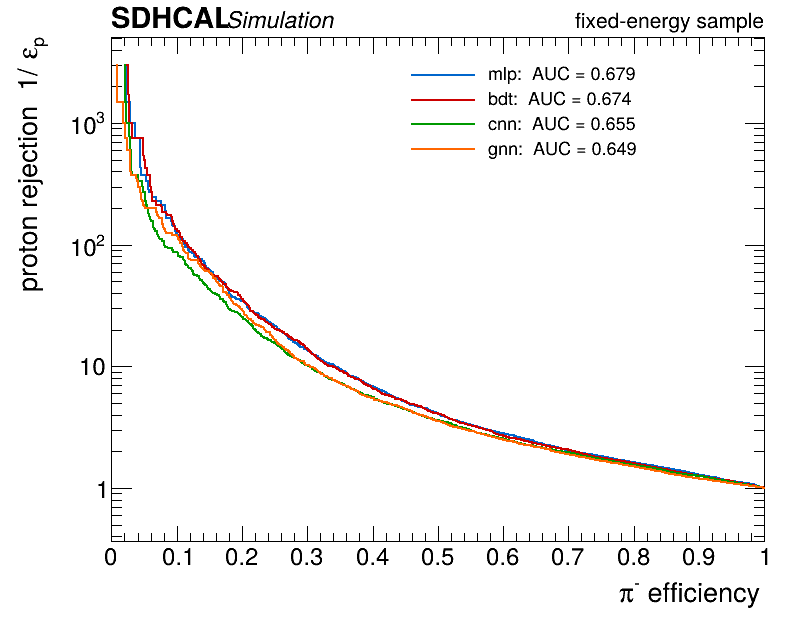
\includegraphics[width=\linewidth]{bench_pid_rejection.png}
    \caption{Proton rejection versus pion efficiency.}
  \end{subfigure}\hfill
  \begin{subfigure}[t]{0.49\textwidth}
    \centering
    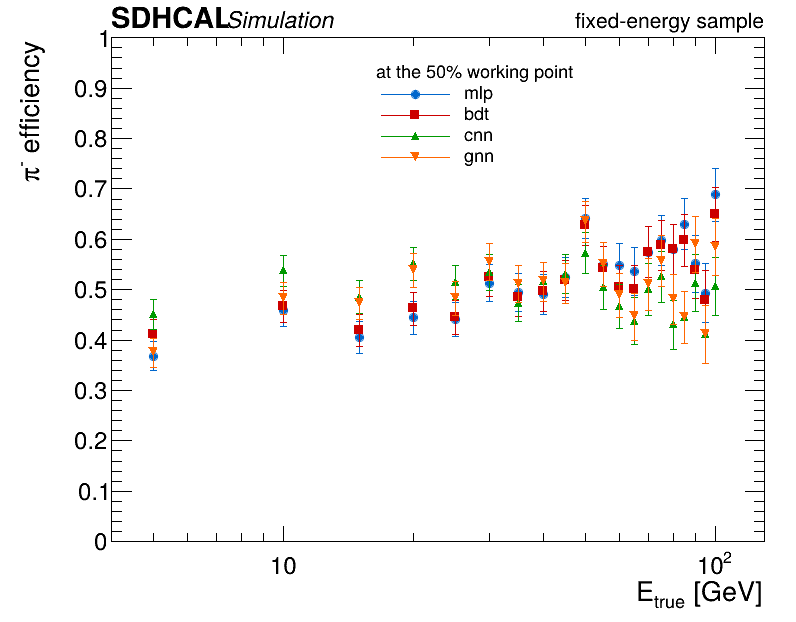
\includegraphics[width=\linewidth]{bench_pid_efficiency.png}
    \caption{Pion efficiency versus true energy at the global 50\% working point.}
  \end{subfigure}
  \caption{External pion--proton identification performance. The internal plot label
  ``cnn'' denotes the point-wise permutation-invariant model described in
  \cref{sec:clusters}; it is PointNet-like and does not convolve neighbouring clusters.}
  \label{fig:pid}
\end{figure}

The MLP and BDT have nearly identical rejection at the 50\% working point. Their AUC
difference is $0.0053\pm0.0022$ from the paired bootstrap. The BDT exceeds the
PointNet-like and GNN models by $0.0188\pm0.0047$ and $0.0252\pm0.0051$, respectively.
The difference between the two cluster-level models is $0.0064\pm0.0048$ and is not
resolved by this sample. The pion efficiency increases only gradually with energy and
the per-energy statistical uncertainties are too large to establish a different model
ordering in individual bins.

Pion--proton separation is expected to be difficult because the electromagnetic
fraction and topology fluctuate strongly in pion showers, while baryon-number
conservation modifies the secondary-particle composition of proton showers
\cite{akchurin1998proton}. The present results demonstrate substantial overlap for the
evaluated models and data budget. They do not establish a model-independent physical
upper bound: the cluster-level models use fewer training events, only one seed is
available for each, and no capacity-matched ablation was performed.

\section{Energy-reconstruction performance}
\label{sec:energy-results}

All energy estimators are compared on the same 100744 contained events from the
fixed-energy production. \Cref{tab:energy} reports the fitted stochastic and constant
terms, the resolution obtained after pooling this particular flat grid of generated
energies, and the largest response deviation. The pooled number is sample-spectrum
dependent and is included only as a compact cross-check; $a$ and $b$ are the primary
figures of merit.

\begin{table}[tb]
  \centering
  \caption{Energy performance on the common contained external sample. ``Correction''
  denotes the target in \cref{eq:ratio}. The pooled $\sigma/E$ depends on the flat
  generated spectrum and is not an intrinsic detector resolution.}
  \label{tab:energy}
  \resizebox{\textwidth}{!}{%
  \begin{tabular}{lrrrrr}
    \toprule
    Estimator & Training events & $a$ [\%] & $b$ [\%] & pooled $\sigma/E$ & $\max|\mathcal{R}-1|$ \\
    \midrule
    DeepSets correction & 79451 & $45.5\pm1.0$ & $6.4\pm0.2$ & 0.1115 & 0.028 \\
    BDT correction & 176000 & $53.7\pm1.0$ & $5.6\pm0.3$ & 0.1197 & 0.052 \\
    BDT direct energy & 176000 & $53.6\pm1.1$ & $5.6\pm0.3$ & 0.1199 & 0.054 \\
    Semi-digital calibration & --- & $54.4\pm1.2$ & $7.0\pm0.3$ & 0.1295 & 0.031 \\
    \bottomrule
  \end{tabular}}
\end{table}

\begin{figure}[tb]
  \centering
  \begin{tikzpicture}
\begin{groupplot}[
  group style={group size=2 by 1,horizontal sep=0.75cm},
  width=0.455\textwidth,
  height=0.37\textwidth,
  xmin=4,xmax=101,
  xmode=log,
  log basis x=10,
  xtick={5,10,20,50,100},
  xticklabels={5,10,20,50,100},
  xlabel={$E_{\mathrm{true}}$ [GeV]},
  grid=both,
  minor grid style={gray!12},
  major grid style={gray!22},
  tick label style={font=\footnotesize},
  label style={font=\small},
  legend style={font=\scriptsize,draw=none,fill=none,row sep=-1pt},
  every axis plot/.append style={mark size=1.7pt},
  error bars/y dir=both,
  error bars/y explicit,
]
\nextgroupplot[
  ylabel={$\sigma(E)/E$},
  ymin=0.06,ymax=0.30,
  legend pos=north east,
]
  \addplot+[blue,only marks,mark=o] table[x=energy,y=resolution,y error=resolution_error]
    {plot_data/energy_deepsets.dat};
  \addlegendentry{DeepSets correction}
  \addplot+[blue,no marks,domain=5:100,samples=100,forget plot]
    {sqrt((0.4545373667^2)/x + 0.0640216038^2)};
  \addplot+[red!75!black,only marks,mark=square*] table[x=energy,y=resolution,y error=resolution_error]
    {plot_data/energy_bdt_direct.dat};
  \addlegendentry{BDT direct}
  \addplot+[red!75!black,no marks,domain=5:100,samples=100,forget plot]
    {sqrt((0.5359014700^2)/x + 0.0559016172^2)};
  \addplot+[green!45!black,only marks,mark=triangle*] table[x=energy,y=resolution,y error=resolution_error]
    {plot_data/energy_bdt_ratio.dat};
  \addlegendentry{BDT correction}
  \addplot+[green!45!black,no marks,domain=5:100,samples=100,forget plot]
    {sqrt((0.5366583202^2)/x + 0.0556849631^2)};
  \addplot+[orange!90!black,only marks,mark=triangle*] table[x=energy,y=resolution,y error=resolution_error]
    {plot_data/energy_chi2.dat};
  \addlegendentry{Semi-digital}
  \addplot+[orange!90!black,no marks,domain=5:100,samples=100,forget plot]
    {sqrt((0.5440617998^2)/x + 0.0697165648^2)};

\nextgroupplot[
  ylabel={$\langle E_{\mathrm{rec}}\rangle/E_{\mathrm{true}}$},
  ymin=0.955,ymax=1.065,
  legend pos=north east,
]
  \addplot+[black,densely dotted,no marks,domain=4:101] {1};
  \addplot+[blue,only marks,mark=o] table[x=energy,y=response,y error=response_error]
    {plot_data/energy_deepsets.dat};
  \addplot+[red!75!black,only marks,mark=square*] table[x=energy,y=response,y error=response_error]
    {plot_data/energy_bdt_direct.dat};
  \addplot+[green!45!black,only marks,mark=triangle*] table[x=energy,y=response,y error=response_error]
    {plot_data/energy_bdt_ratio.dat};
  \addplot+[orange!90!black,only marks,mark=triangle*] table[x=energy,y=response,y error=response_error]
    {plot_data/energy_chi2.dat};
\end{groupplot}
\end{tikzpicture}

  \caption{Energy resolution (left) and mean response (right) on the fixed-energy
  sample. Error bars are statistical. The curves in the resolution panel show fits to
  \cref{eq:resolution}. The source artifact historically named \texttt{gnn\_ratio}
  is labelled DeepSets here because the retained run uses no graph edges.}
  \label{fig:energy}
\end{figure}

The BDT variants and the semi-digital calibration have compatible stochastic terms
near 54\%. The improvement of the BDT over the calibration is concentrated in the
constant term, which decreases from $(7.0\pm0.3)\%$ to $(5.6\pm0.3)\%$. Changing the
BDT target from direct energy to the correction of \cref{eq:ratio} has no significant
effect.

The DeepSets correction instead decreases the stochastic term to $(45.5\pm1.0)\%$.
It gives the best resolution over the complete evaluated range and keeps the maximum
response deviation below 2.9\%. Because DeepSets contains no graph edges, this gain
cannot be attributed to explicit cluster connectivity. It is evidence that the
cluster-level representation and learned aggregation contain useful event-wise
information beyond the threshold counts and selected global descriptors.

A control model trained directly on $\log E$ reached a pooled resolution of 0.203 and
a stochastic term near 78\%, while its response changed from approximately 1.21 at
5~\GeV{} to 0.81 at 100~\GeV{}. This regression-to-the-mean behaviour motivates the
ratio target in \cref{eq:ratio}. Conversely, applying the ratio target to the BDT does
not improve its result, which indicates that the DeepSets gain is not explained by the
target transformation alone.

\section{Does explicit particle identification improve energy reconstruction?}
\label{sec:coupling}

The downstream effect of particle identification is isolated by crossing three label
sources with two estimator families. The label is either absent, supplied by the BDT
classifier, or set to the true species as an oracle. Without a label, the parametric
method uses pion coefficients for every event, whereas the learned method uses one
inclusive BDT trained on the pion--proton mixture. With a predicted or true label,
species-specific parametric calibrations or BDT regressors are selected.

\begin{table}[tb]
  \centering
  \caption{Global mean bias and resolution for the coupled PID--energy study. All
  scenarios use the containment selection. Predicted-label rows contain 100678 events;
  the other rows contain 100744.}
  \label{tab:coupling}
  \begin{tabular}{llrr}
    \toprule
    Label source & Energy estimator & Mean bias [\%] & $\sigma/E$ \\
    \midrule
    none (pion reference) & semi-digital & $-1.36$ & 0.1342 \\
    predicted BDT label & semi-digital & $+0.60$ & 0.1287 \\
    true label & semi-digital & $-0.27$ & 0.1295 \\
    \midrule
    none (inclusive) & BDT & $+2.00$ & 0.1199 \\
    predicted BDT label & BDT & $+2.02$ & 0.1201 \\
    true label & BDT & $+1.88$ & 0.1199 \\
    \bottomrule
  \end{tabular}
\end{table}

Species routing improves the parametric result relative to applying pion coefficients
to all events. This comparison mainly corrects a mismatched proton calibration and
should not be interpreted as an absolute gain from PID. Once the baseline is an
inclusive BDT trained on the mixture, no improvement is observed: the resolutions
without a label, with the predicted label, and with the true label are 0.1199, 0.1201,
and 0.1199. Their statistical uncertainties are approximately $3\times10^{-4}$, and
the inclusive BDT has a seed-to-seed spread of 0.0008 over five seeds.

In this setting, the global shower descriptors already contain the information that
the explicit species label would provide. Routing replaces this continuous information
with a hard binary decision and therefore adds no measurable resolution. This result
is conditional on the balanced pion--proton mixture, the simulated detector, and the
trained energy range. It need not hold for a strongly shifted particle composition,
an unseen species, or detector data with different feature resolutions.

\section{Discussion and limitations}
\label{sec:limitations}

The study supports two distinct conclusions. First, under the available training
budgets, global shower descriptors are at least as effective as the tested cluster
graph for pion--proton identification. The unequal budgets prevent attributing the
difference solely to representation or architecture. Second, cluster-level information
does improve energy reconstruction when used by the DeepSets correction. This finding
does not demonstrate a benefit from graph connectivity; a direct, budget-matched
comparison between DeepSets, a static graph, and a dynamic graph remains necessary.

Several limitations define the scope of the numerical results:
\begin{itemize}
  \item all samples are simulated, with no beam-test validation or detector-model
        systematic uncertainty;
  \item the simulation configuration was recovered from copied build files, launch
        scripts, and logs rather than from immutable metadata embedded in the event
        files; the production scripts and local extraction changes must be archived
        with content hashes before submission;
  \item pion and proton jobs share deterministic seed schedules, and the digitisation
        jobs reuse a fixed random seed; the effect of the resulting correlations has
        not been quantified;
  \item parallel digitisation jobs contended for a shared auxiliary AIDA output. The
        logs report successful LCIO completion for all 40 fixed-energy shards per
        species, but the diagnostic-file write failures should be eliminated in any
        reproduced production;
  \item the \SI{0.1}{ns} timing smearing is assumed, and no timing ablation is included
        in the retained benchmark;
  \item the containment selection changes from 95.8\% to 23.1\% across the energy
        range and preferentially retains compact high-energy showers;
  \item the DeepSets result corresponds to one training seed, whereas a five-seed
        spread is available only for the inclusive BDT;
  \item the PID comparison uses a model-dependent common intersection of 6027 events
        and markedly different training budgets;
  \item the quoted uncertainties are statistical and do not cover hadronic-model,
        calibration, efficiency, threshold, noise, or alignment variations.
\end{itemize}

These limitations are particularly important when comparing with published DHCAL or
HGCAL results. Differences in absorber depth, active medium, analogue versus digital
readout, leakage treatment, particle composition, and core-width definition preclude
a direct numerical ranking~\cite{borysova2025dhcalgnn,aamir2024hgcalgnn}.

\section{Reproducibility}
\label{sec:reproducibility}

The analysis keeps the continuous production for training and internal calibration
and the fixed-energy production for external evaluation. Geant4 10.04.p03 and
QGSP\_BERT are confirmed by the retained fixed-energy production logs and the copied
executable build tree; all four particle-production launchers select the same physics
list. Analysis random seeds, feature order, event identifiers, containment flags,
model metadata, and event-level predictions are recorded by the software workflow.
The simulation seed schedule is retained in the launch scripts but is not embedded in
the event files.

The article tables are frozen from the common benchmark outputs, and the energy curves
in \cref{fig:energy} are stored as plain-text data beside this source. The software
repository URL, an immutable archive of the exact local simulation and extraction
sources, and an archival DOI will be added before submission. The simulated event
samples are not included in the source repository; their access and preservation
policy must be agreed by the authors and the relevant collaboration.

\section{Conclusion}
\label{sec:conclusion}

Binary pion--proton identification and hadron energy reconstruction have been studied
with separate training and fixed-energy evaluation productions in a simulated
semi-digital calorimeter. On a common external subset, an MLP and a LightGBM classifier
using shower descriptors reach AUC values of 0.679 and 0.674. A PointNet-like cluster
model and a static GNN reach 0.655 and 0.649 with twenty times fewer training events;
the comparison therefore motivates, but does not replace, a budget-matched study.

For energy reconstruction, a particle-blind DeepSets correction to the three-threshold
calibration reduces the fitted stochastic term from $(54.4\pm1.2)\%$ to
$(45.5\pm1.0)\%$ on contained showers. The corresponding constant term is
$(6.4\pm0.2)\%$. An inclusive boosted-tree regressor is not improved by adding either
the predicted or true pion--proton label, showing that explicit PID routing is
redundant for that estimator in the evaluated mixture. Validation on beam-test data,
simulation systematics, repeated neural-network training, and controlled comparisons
of set and graph architectures are required before drawing an experimental conclusion.

\section*{Acknowledgements}

The acknowledgement text, funding identifiers, computing resources, and collaboration
approval statement will be completed jointly by the authors before submission.

\printbibliography

\end{document}
